\section{Introduction}
Welcome to our guide for metamodeling with \textbf{eMoflon::IBeX}. In the first part of the tutorial we will show you how to install the required software for using eMoflon::IBeX and how to create your first metamodel.\newline
The second part of our tutorial will teach you the functions of \textbf{eMoflon::IBeX-GT} our interpreter for graph transformation rules, that employs various incremental graph pattern matching tools to provide solid performance, even on large-scale models.\newline
The third and final part is focused on bidirectional model transformation with \textbf{triple grammar graphs}.\newline
There are almost no prerequisites to tackle this tutorial. The only thing you might need is some basic knowledge of Eclipse and programming with Java. A fundamental understanding of metamodeling might come in handy but is not required. 

\section{Install instructions}

\raggedright

\subsection{General}

\textbf{Eclipse Modelling Tools:}

First of all you need a running version of \textbf{Eclipse} that includes the \textbf{Eclipse Modelling Tools} package.

You can install it by running the regular Eclipse installer and choosing \textbf{Eclipse Modeling Tools} in the installation wizard. Afterwards just follow the instructions.\newline
You can download the newest installer \underline{\href{https://www.eclipse.org/downloads/}{here}}.\newline

\textbf{Eclipse Modelling Framework:}

The Eclipse Modelling Tools version you just installed includes, among other features, a set of plug-ins for Eclipse which enable the modulation of data models, the generation of corresponding code, and outputs based on this model.\newline
This set of plug-ins is summarized under the name \textbf{Eclipse Modelling Framework (EMF)}.\newline
The user can create metamodels via different means such as UML or XML schemes. The metamodels created with EMF consist of two parts: the \textbf{ecore} and the \textbf{genmodel} description files which you will get to know better throughout this tutorial\footnote{\href{https://www.vogella.com/tutorials/EclipseEMF/article.html}{See: Vogella EclipseEMF article \underline{here}}}.

\subsection{Windows specific}

\textbf{GraphViz:}

Another standalone software you will need for the visualization of the created metamodels is \textbf{GraphViz}.

You can download the newest installers for Windows \href{https://graphviz.org/download/}{\underline{here}}.

Just follow the install instructions from the installer.\newline

You can continue with step \textbf{2.4} now.
\subsection{Linux specific}

\textbf{GraphViz:}

Another standalone software you will need for the visualization of the created metamodels is \textbf{GraphViz}. On Linux it is requiered to install the corresponding package.\newline You can look at an overview for the different Linux plattforms \href{https://graphviz.org/download/}{\underline{here}}.

\clearpage

\subsection{Eclipse plugins}

\textbf{PlantUML:}

If you have completed the previous section, you are ready to install the remaining software in Eclipse. You will also need \textsf{\textit{PlantUML}} for the visualization of our class diagrams. The easiest way to install this plugin is to use the integrated \textbf{Eclipse Marketplace}.

The \textsf{\textit{Marketplace}} can be accessed over:\newline

\centering
→ \textsf{\textit{Help}} drop-down menu →
\textsf{\textit{Eclipse Marketplace}}\newline

\raggedright
A new window should pop up, which presents an overview of available software plugins. Now type \textit{\textsf{PlantUML}} in the search window on the very top and install \textbf{the PlantUML plugin}.The chart below provides a cumulated view of the previous steps.\newline\newline

\begin{figure}[h]
    \centering
    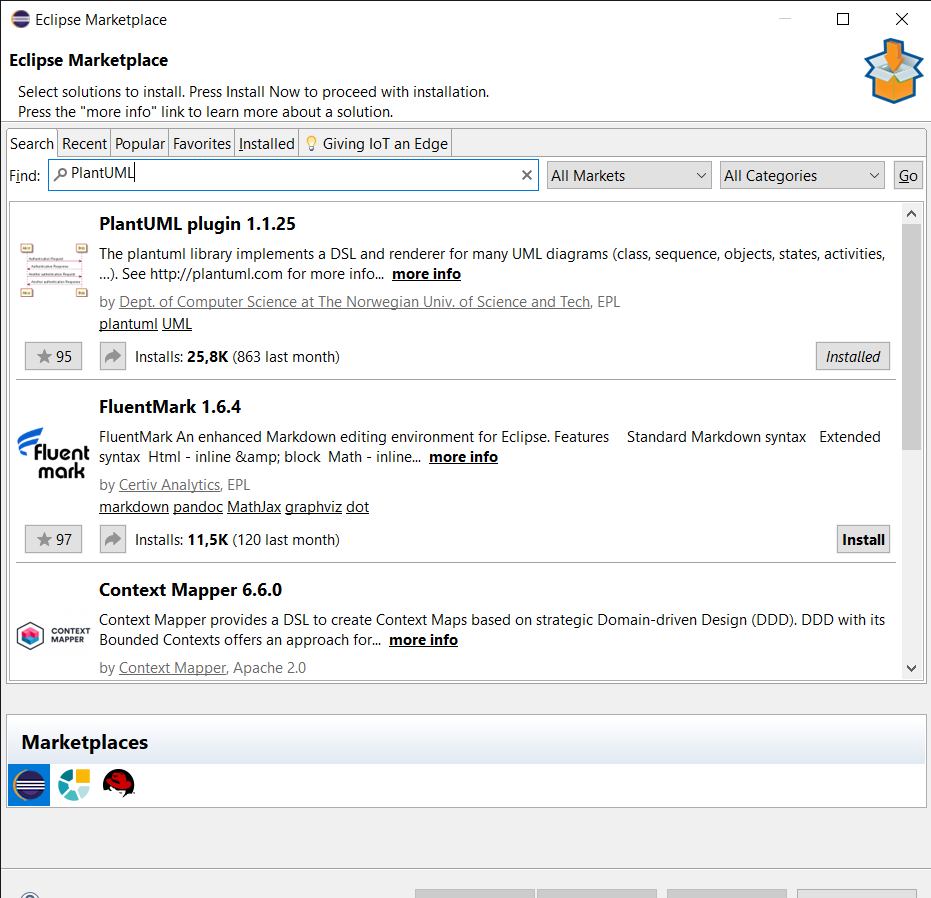
\includegraphics[scale = 0.4]{pictures/Eclipse Marketplace 08.11.2021 16_56_39.png}
    \label{screenshot marketplace}
    \caption{\centering{Screenshot of the \textit{Marketplace}}}
    
\end{figure}
\clearpage
\textbf{HiPE}: \newline\newline
You also need to install the plugin \textsf{\textit{HiPe}} beforehand. You need to click: \newline

\centering
→ \textsf{\textit{Help}} →
\textsf{\textit{Install New Software}}\newline

\raggedright
Another window should pop up and you can insert the following URL into the \textsf{\textit{Work with}} field:\newline


\centering
{\color{blue}https://hipe-devops.github.io/HiPE-Updatesite/hipe.updatesite/ \newline}

\raggedright
After pressing \textsf{\textit{Enter}} you should now see the window from the chart below presenting \textsf{\textit{HiPE}} next to a checkbox. Start the installation by selecting it, clicking \textsf{\textit{next}}, accepting the license agreement, and pressing \textsf{\textit{install anyway}} afterward. Throughout the process of installing Eclipse may require a restart. If Eclipse restarts without any errors, everything necessary is installed.\newline\newline

\begin{figure}[h]
    \centering
    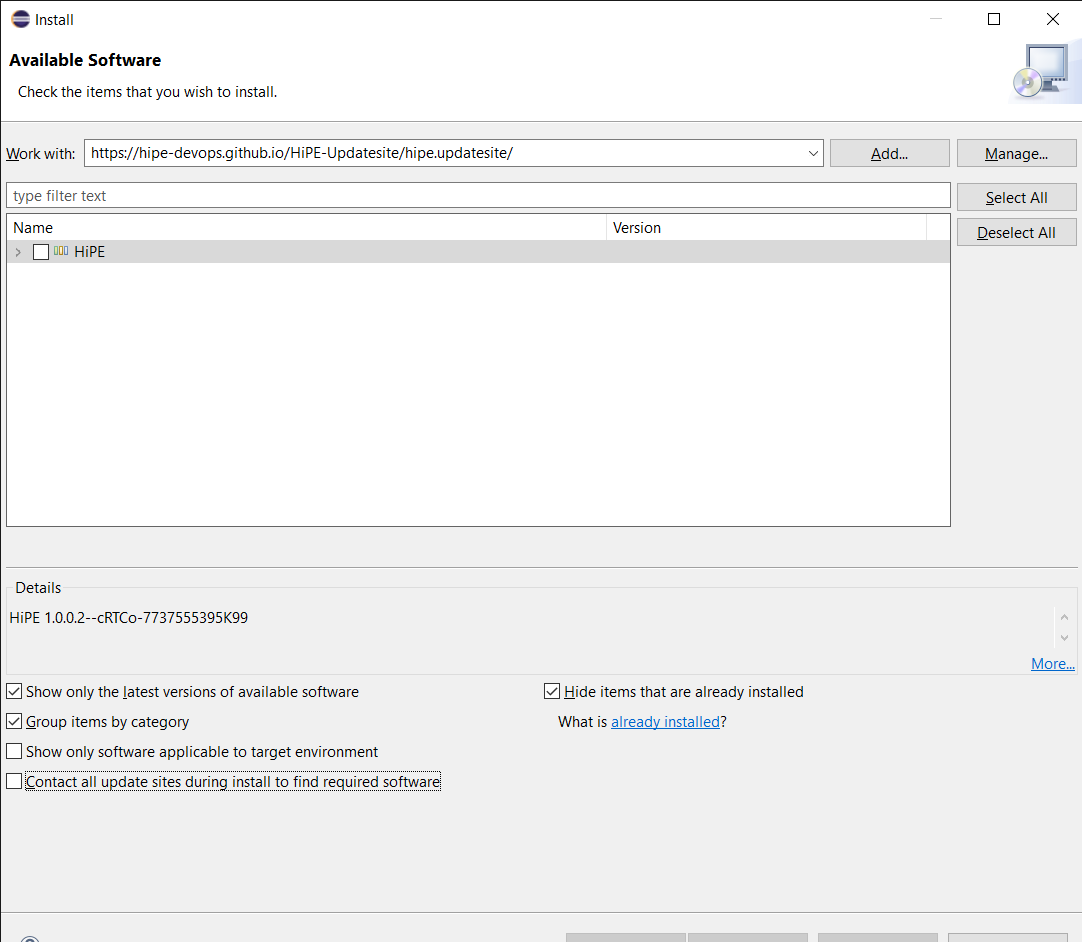
\includegraphics[scale=0.5]{pictures/eclipse_install_new_software_hipe.png}
    \caption{\centering{Screenshot of the \textit{Install New Software} window for \textsf{\textit{HiPE}}}}
    \label{screenshot install new software hipe}
\end{figure}

\clearpage

\textbf{eMoflon::IBeX:}\newline\newline
Now we will install \textbf{eMoflon::IBeX}. This is done in the same way as the \textsf{\textit{HiPE}} plugin. You can insert the following URL into the \textsf{\textit{Work with}} field:\newline

\centering
{\color{blue}https://emoflon.org/emoflon-ibex-updatesite/snapshot/updatesite/\newline}


\raggedright
You should now see the window from the chart below presenting \textsf{\textit{eMoflon:IBeX}} and it's different submodules. For this tutorial you will need \textsf{\textit{Democles}} and \textsf{\textit{HiPE}}. Although installing the whole suite does no harm.

Continue with the installation in the same way as in the previous step.\newline

\begin{figure}[h]
    \centering
    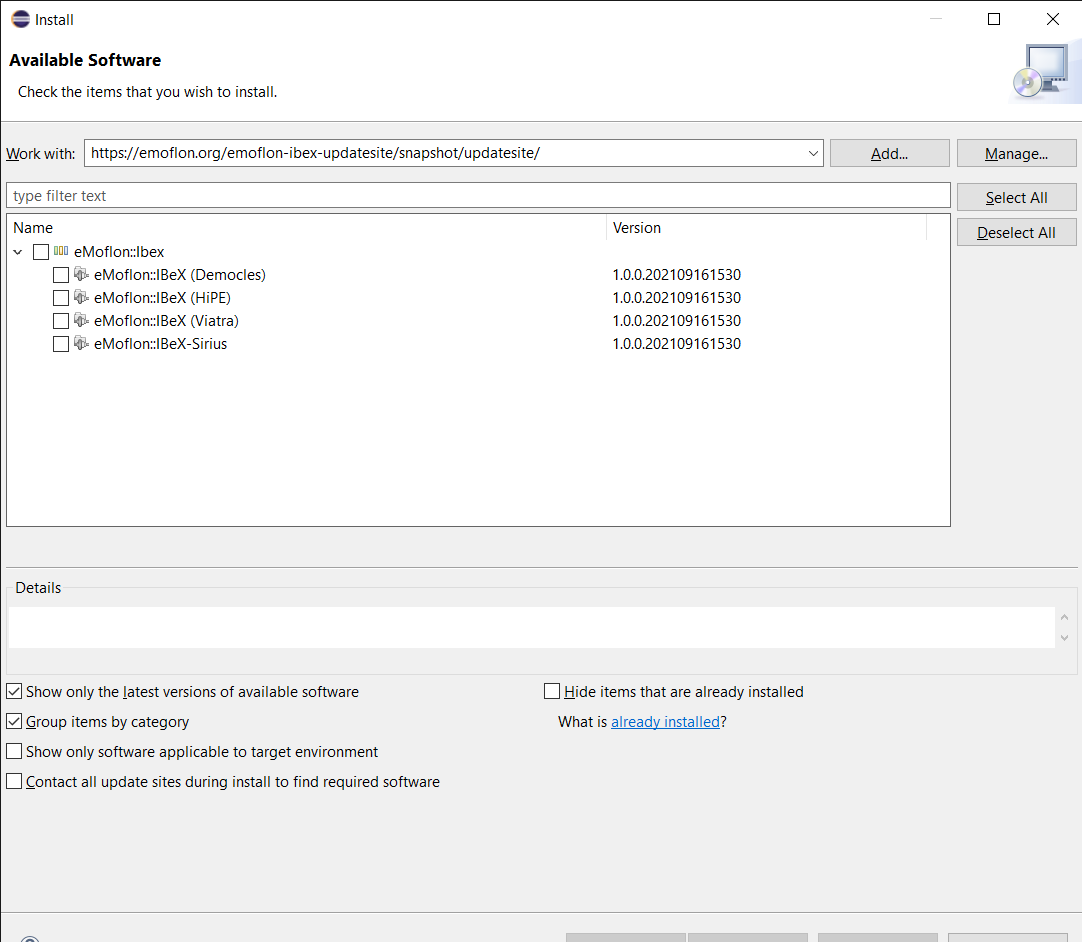
\includegraphics[scale=0.4, width =\textwidth]{pictures/eclipse-workspace - HospitalExample_model_HospitalExample.ecore - Eclipse IDE 08.11.2021 18_02_54.png}
    \caption{\centering{Screenshot of the \textit{\textsf{Install New Software}} window for \textit{\textsf{eMoflon::IBeX}}}}
    \label{screenshot install new software eMoflon::IBeX}
\end{figure}

Both \textsf{\textit{Democles}} and \textsf{\textit{HiPE}} are Eclipse projects which include pattern matching engines.

%\textsf{\textit{Viatra}} provides a framework with an editor for model queries and a code generator to implement the model queries easily into java code.
% ^Viatra is now deprecated (within eMoflon context)

\textsf{\textit{Sirius}} is a framework for visualization which implements a graphic editor for triple graph grammar rules.\newline 

In this tutorial we will just need the incremental pattern matchers the first two. In contrast to \textsf{\textit{Democles}} \textsf{\textit{HiPE}} is a parallel pattern matcher.

\clearpage